% Created by tikzDevice version 0.12.6 on 2025-05-06 20:54:35
% !TEX encoding = UTF-8 Unicode
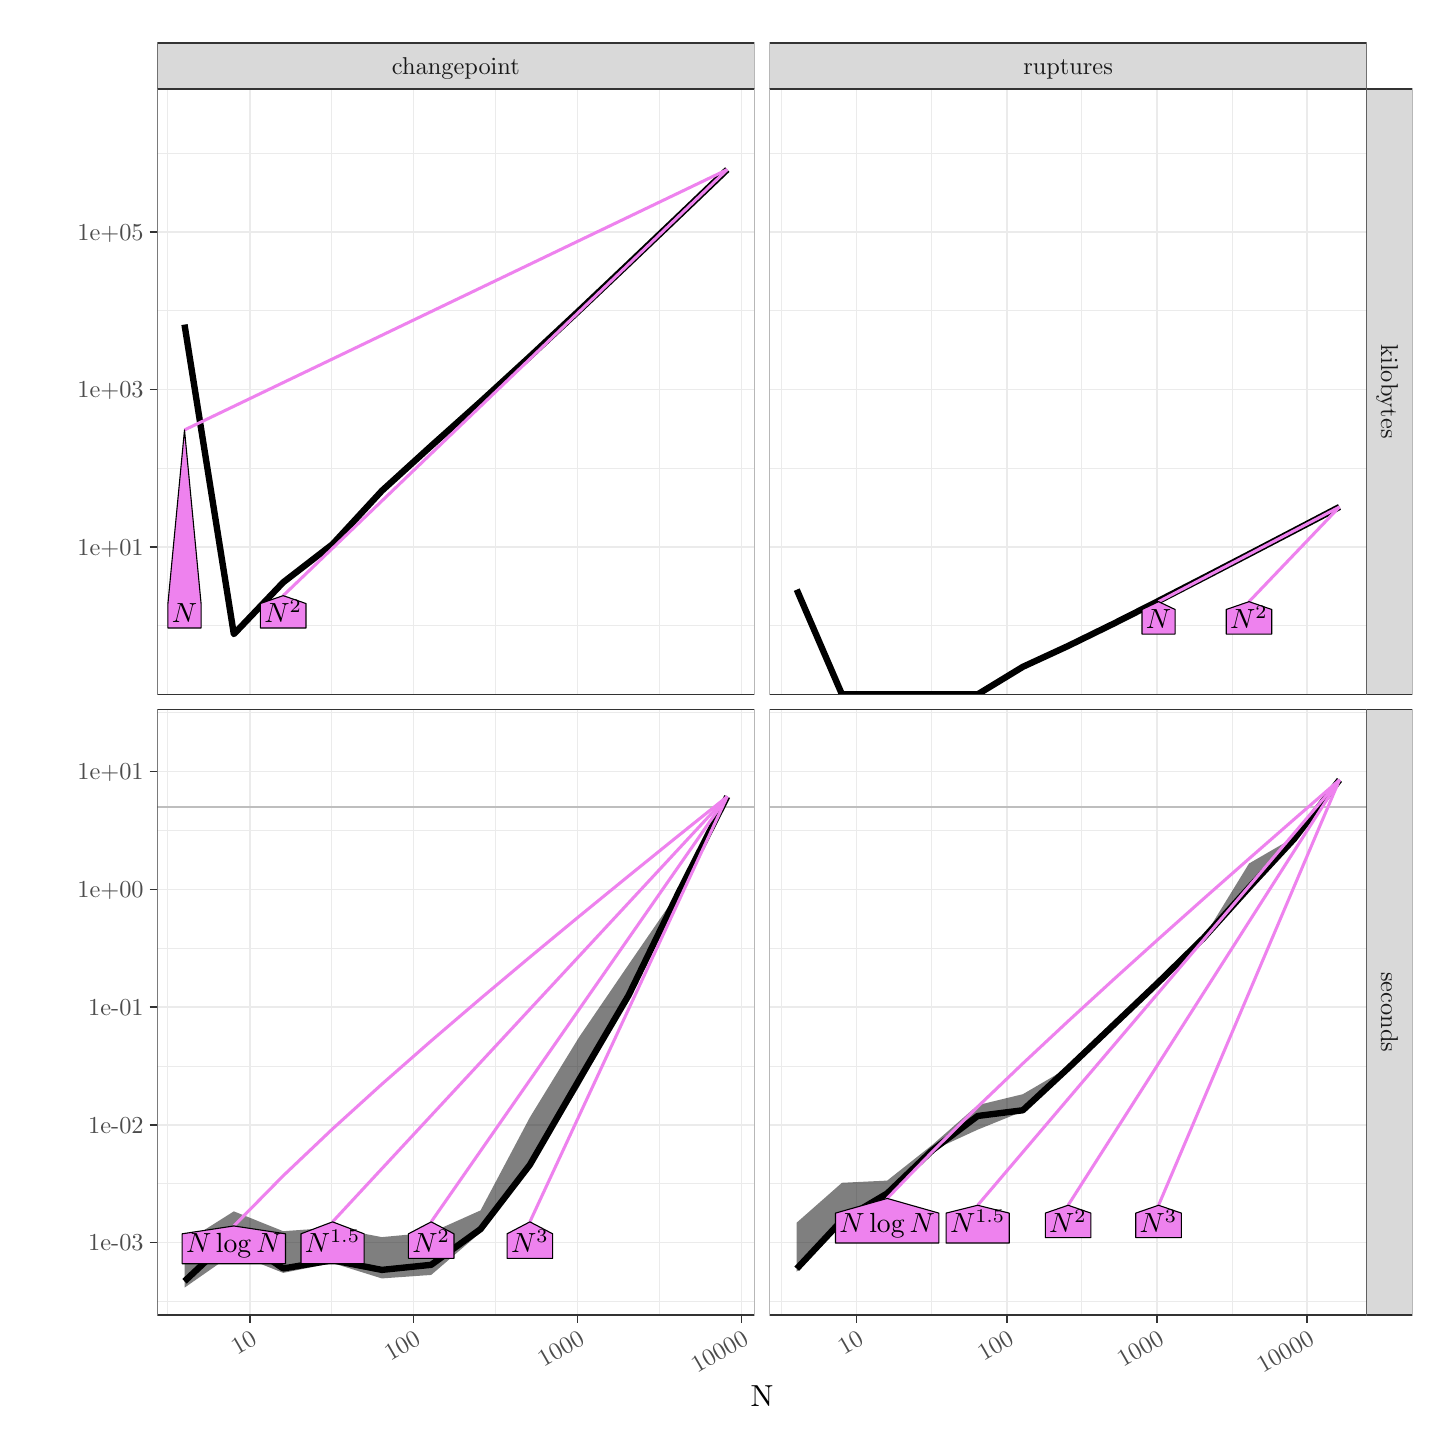
\begin{tikzpicture}[x=1pt,y=1pt]
\definecolor{fillColor}{RGB}{255,255,255}
\path[use as bounding box,fill=fillColor,fill opacity=0.00] (0,0) rectangle (505.89,505.89);
\begin{scope}
\path[clip] (  0.00,  0.00) rectangle (505.89,505.89);
\definecolor{drawColor}{RGB}{255,255,255}
\definecolor{fillColor}{RGB}{255,255,255}

\path[draw=drawColor,line width= 0.6pt,line join=round,line cap=round,fill=fillColor] (  0.00,  0.00) rectangle (505.89,505.89);
\end{scope}
\begin{scope}
\path[clip] ( 46.86,264.98) rectangle (262.59,483.82);
\definecolor{fillColor}{RGB}{255,255,255}

\path[fill=fillColor] ( 46.86,264.98) rectangle (262.59,483.82);
\definecolor{drawColor}{gray}{0.92}

\path[draw=drawColor,line width= 0.3pt,line join=round] ( 46.86,289.91) --
	(262.59,289.91);

\path[draw=drawColor,line width= 0.3pt,line join=round] ( 46.86,346.74) --
	(262.59,346.74);

\path[draw=drawColor,line width= 0.3pt,line join=round] ( 46.86,403.56) --
	(262.59,403.56);

\path[draw=drawColor,line width= 0.3pt,line join=round] ( 46.86,460.39) --
	(262.59,460.39);

\path[draw=drawColor,line width= 0.3pt,line join=round] ( 50.63,264.98) --
	( 50.63,483.82);

\path[draw=drawColor,line width= 0.3pt,line join=round] (109.85,264.98) --
	(109.85,483.82);

\path[draw=drawColor,line width= 0.3pt,line join=round] (169.08,264.98) --
	(169.08,483.82);

\path[draw=drawColor,line width= 0.3pt,line join=round] (228.30,264.98) --
	(228.30,483.82);

\path[draw=drawColor,line width= 0.6pt,line join=round] ( 46.86,318.33) --
	(262.59,318.33);

\path[draw=drawColor,line width= 0.6pt,line join=round] ( 46.86,375.15) --
	(262.59,375.15);

\path[draw=drawColor,line width= 0.6pt,line join=round] ( 46.86,431.98) --
	(262.59,431.98);

\path[draw=drawColor,line width= 0.6pt,line join=round] ( 80.24,264.98) --
	( 80.24,483.82);

\path[draw=drawColor,line width= 0.6pt,line join=round] (139.46,264.98) --
	(139.46,483.82);

\path[draw=drawColor,line width= 0.6pt,line join=round] (198.69,264.98) --
	(198.69,483.82);

\path[draw=drawColor,line width= 0.6pt,line join=round] (257.92,264.98) --
	(257.92,483.82);
\definecolor{drawColor}{RGB}{0,0,0}

\path[draw=drawColor,line width= 2.3pt,line join=round] ( 56.67,398.60) --
	( 74.50,286.74) --
	( 92.33,305.45) --
	(110.16,319.22) --
	(127.98,338.53) --
	(145.81,354.75) --
	(163.64,370.70) --
	(181.47,387.04) --
	(199.30,403.70) --
	(217.13,420.58) --
	(234.96,437.56) --
	(252.79,454.61);
\definecolor{drawColor}{RGB}{238,130,238}

\path[draw=drawColor,line width= 1.1pt,line join=round] ( 92.33,300.65) --
	(110.16,317.76) --
	(127.98,334.86) --
	(145.81,351.97) --
	(163.64,369.07) --
	(181.47,386.18) --
	(199.30,403.29) --
	(217.13,420.39) --
	(234.96,437.50) --
	(252.79,454.61);

\path[draw=drawColor,line width= 1.1pt,line join=round] ( 56.67,360.52) --
	( 74.50,369.07) --
	( 92.33,377.63) --
	(110.16,386.18) --
	(127.98,394.73) --
	(145.81,403.29) --
	(163.64,411.84) --
	(181.47,420.39) --
	(199.30,428.95) --
	(217.13,437.50) --
	(234.96,446.05) --
	(252.79,454.61);
\end{scope}
\begin{scope}
\path[clip] ( 46.86,264.98) rectangle (262.59,483.82);
\definecolor{drawColor}{RGB}{0,0,0}
\definecolor{fillColor}{RGB}{238,130,238}

\path[draw=drawColor,line width= 0.4pt,line join=round,line cap=round,fill=fillColor] ( 84.10,297.80) --
	( 92.33,300.65) --
	(100.56,297.80) --
	(100.56,288.94) --
	( 84.10,288.94) --
	cycle;

\path[draw=drawColor,line width= 0.4pt,line join=round,line cap=round,fill=fillColor] ( 50.68,297.80) --
	( 56.67,360.52) --
	( 62.66,297.80) --
	( 62.66,288.94) --
	( 50.68,288.94) --
	cycle;

\node[text=drawColor,anchor=base,inner sep=0pt, outer sep=0pt, scale=  1.00] at ( 92.33,290.92) {$N^2$};

\node[text=drawColor,anchor=base,inner sep=0pt, outer sep=0pt, scale=  1.00] at ( 56.67,290.92) {$N$};
\definecolor{drawColor}{gray}{0.20}

\path[draw=drawColor,line width= 0.6pt,line join=round,line cap=round] ( 46.86,264.98) rectangle (262.59,483.82);
\end{scope}
\begin{scope}
\path[clip] ( 46.86, 40.64) rectangle (262.59,259.48);
\definecolor{fillColor}{RGB}{255,255,255}

\path[fill=fillColor] ( 46.86, 40.64) rectangle (262.59,259.48);
\definecolor{drawColor}{gray}{0.92}

\path[draw=drawColor,line width= 0.3pt,line join=round] ( 46.86, 45.62) --
	(262.59, 45.62);

\path[draw=drawColor,line width= 0.3pt,line join=round] ( 46.86, 88.17) --
	(262.59, 88.17);

\path[draw=drawColor,line width= 0.3pt,line join=round] ( 46.86,130.71) --
	(262.59,130.71);

\path[draw=drawColor,line width= 0.3pt,line join=round] ( 46.86,173.25) --
	(262.59,173.25);

\path[draw=drawColor,line width= 0.3pt,line join=round] ( 46.86,215.80) --
	(262.59,215.80);

\path[draw=drawColor,line width= 0.3pt,line join=round] ( 46.86,258.34) --
	(262.59,258.34);

\path[draw=drawColor,line width= 0.3pt,line join=round] ( 50.63, 40.64) --
	( 50.63,259.48);

\path[draw=drawColor,line width= 0.3pt,line join=round] (109.85, 40.64) --
	(109.85,259.48);

\path[draw=drawColor,line width= 0.3pt,line join=round] (169.08, 40.64) --
	(169.08,259.48);

\path[draw=drawColor,line width= 0.3pt,line join=round] (228.30, 40.64) --
	(228.30,259.48);

\path[draw=drawColor,line width= 0.6pt,line join=round] ( 46.86, 66.89) --
	(262.59, 66.89);

\path[draw=drawColor,line width= 0.6pt,line join=round] ( 46.86,109.44) --
	(262.59,109.44);

\path[draw=drawColor,line width= 0.6pt,line join=round] ( 46.86,151.98) --
	(262.59,151.98);

\path[draw=drawColor,line width= 0.6pt,line join=round] ( 46.86,194.52) --
	(262.59,194.52);

\path[draw=drawColor,line width= 0.6pt,line join=round] ( 46.86,237.07) --
	(262.59,237.07);

\path[draw=drawColor,line width= 0.6pt,line join=round] ( 80.24, 40.64) --
	( 80.24,259.48);

\path[draw=drawColor,line width= 0.6pt,line join=round] (139.46, 40.64) --
	(139.46,259.48);

\path[draw=drawColor,line width= 0.6pt,line join=round] (198.69, 40.64) --
	(198.69,259.48);

\path[draw=drawColor,line width= 0.6pt,line join=round] (257.92, 40.64) --
	(257.92,259.48);
\definecolor{drawColor}{RGB}{190,190,190}

\path[draw=drawColor,line width= 0.6pt,line join=round] ( 46.86,224.26) -- (262.59,224.26);
\definecolor{fillColor}{RGB}{0,0,0}

\path[fill=fillColor,fill opacity=0.50] ( 56.67, 66.89) --
	( 74.50, 78.17) --
	( 92.33, 71.00) --
	(110.16, 72.26) --
	(127.98, 68.86) --
	(145.81, 70.52) --
	(163.64, 78.50) --
	(181.47,112.13) --
	(199.30,141.19) --
	(217.13,167.33) --
	(234.96,193.27) --
	(252.79,228.18) --
	(252.79,227.94) --
	(234.96,192.75) --
	(217.13,155.33) --
	(199.30,123.25) --
	(181.47, 94.27) --
	(163.64, 70.55) --
	(145.81, 55.19) --
	(127.98, 53.93) --
	(110.16, 59.50) --
	( 92.33, 55.94) --
	( 74.50, 63.02) --
	( 56.67, 50.59) --
	cycle;

\path[] ( 56.67, 66.89) --
	( 74.50, 78.17) --
	( 92.33, 71.00) --
	(110.16, 72.26) --
	(127.98, 68.86) --
	(145.81, 70.52) --
	(163.64, 78.50) --
	(181.47,112.13) --
	(199.30,141.19) --
	(217.13,167.33) --
	(234.96,193.27) --
	(252.79,228.18);

\path[] (252.79,227.94) --
	(234.96,192.75) --
	(217.13,155.33) --
	(199.30,123.25) --
	(181.47, 94.27) --
	(163.64, 70.55) --
	(145.81, 55.19) --
	(127.98, 53.93) --
	(110.16, 59.50) --
	( 92.33, 55.94) --
	( 74.50, 63.02) --
	( 56.67, 50.59);
\definecolor{drawColor}{RGB}{0,0,0}

\path[draw=drawColor,line width= 2.3pt,line join=round] ( 56.67, 52.89) --
	( 74.50, 69.63) --
	( 92.33, 57.53) --
	(110.16, 60.50) --
	(127.98, 57.01) --
	(145.81, 58.85) --
	(163.64, 71.74) --
	(181.47, 94.98) --
	(199.30,125.79) --
	(217.13,156.20) --
	(234.96,192.85) --
	(252.79,228.05);
\definecolor{drawColor}{RGB}{238,130,238}

\path[draw=drawColor,line width= 1.1pt,line join=round] ( 74.50, 72.89) --
	( 92.33, 91.02) --
	(110.16,107.95) --
	(127.98,124.12) --
	(145.81,139.78) --
	(163.64,155.05) --
	(181.47,170.03) --
	(199.30,184.79) --
	(217.13,199.35) --
	(234.96,213.77) --
	(252.79,228.05);

\path[draw=drawColor,line width= 1.1pt,line join=round] (110.16, 74.37) --
	(127.98, 93.58) --
	(145.81,112.79) --
	(163.64,132.00) --
	(181.47,151.21) --
	(199.30,170.42) --
	(217.13,189.63) --
	(234.96,208.84) --
	(252.79,228.05);

\path[draw=drawColor,line width= 1.1pt,line join=round] (145.81, 74.37) --
	(163.64, 99.99) --
	(181.47,125.60) --
	(199.30,151.21) --
	(217.13,176.83) --
	(234.96,202.44) --
	(252.79,228.05);

\path[draw=drawColor,line width= 1.1pt,line join=round] (181.47, 74.37) --
	(199.30,112.79) --
	(217.13,151.21) --
	(234.96,189.63) --
	(252.79,228.05);
\end{scope}
\begin{scope}
\path[clip] ( 46.86, 40.64) rectangle (262.59,259.48);
\definecolor{drawColor}{RGB}{0,0,0}
\definecolor{fillColor}{RGB}{238,130,238}

\path[draw=drawColor,line width= 0.4pt,line join=round,line cap=round,fill=fillColor] ( 55.83, 70.05) --
	( 74.50, 72.89) --
	( 93.17, 70.05) --
	( 93.17, 59.24) --
	( 55.83, 59.24) --
	cycle;

\path[draw=drawColor,line width= 0.4pt,line join=round,line cap=round,fill=fillColor] ( 98.75, 70.05) --
	(110.16, 74.37) --
	(121.56, 70.05) --
	(121.56, 59.24) --
	( 98.75, 59.24) --
	cycle;

\path[draw=drawColor,line width= 0.4pt,line join=round,line cap=round,fill=fillColor] (137.59, 70.05) --
	(145.81, 74.37) --
	(154.04, 70.05) --
	(154.04, 61.18) --
	(137.59, 61.18) --
	cycle;

\path[draw=drawColor,line width= 0.4pt,line join=round,line cap=round,fill=fillColor] (173.24, 70.05) --
	(181.47, 74.37) --
	(189.70, 70.05) --
	(189.70, 61.18) --
	(173.24, 61.18) --
	cycle;

\node[text=drawColor,anchor=base,inner sep=0pt, outer sep=0pt, scale=  1.00] at ( 74.50, 63.16) {$N \log N$};

\node[text=drawColor,anchor=base,inner sep=0pt, outer sep=0pt, scale=  1.00] at (110.16, 63.16) {$N^{1.5}$};

\node[text=drawColor,anchor=base,inner sep=0pt, outer sep=0pt, scale=  1.00] at (145.81, 63.16) {$N^2$};

\node[text=drawColor,anchor=base,inner sep=0pt, outer sep=0pt, scale=  1.00] at (181.47, 63.16) {$N^3$};
\definecolor{drawColor}{gray}{0.20}

\path[draw=drawColor,line width= 0.6pt,line join=round,line cap=round] ( 46.86, 40.64) rectangle (262.59,259.48);
\end{scope}
\begin{scope}
\path[clip] (268.09,264.98) rectangle (483.82,483.82);
\definecolor{fillColor}{RGB}{255,255,255}

\path[fill=fillColor] (268.09,264.98) rectangle (483.82,483.82);
\definecolor{drawColor}{gray}{0.92}

\path[draw=drawColor,line width= 0.3pt,line join=round] (268.09,289.91) --
	(483.82,289.91);

\path[draw=drawColor,line width= 0.3pt,line join=round] (268.09,346.74) --
	(483.82,346.74);

\path[draw=drawColor,line width= 0.3pt,line join=round] (268.09,403.56) --
	(483.82,403.56);

\path[draw=drawColor,line width= 0.3pt,line join=round] (268.09,460.39) --
	(483.82,460.39);

\path[draw=drawColor,line width= 0.3pt,line join=round] (272.36,264.98) --
	(272.36,483.82);

\path[draw=drawColor,line width= 0.3pt,line join=round] (326.65,264.98) --
	(326.65,483.82);

\path[draw=drawColor,line width= 0.3pt,line join=round] (380.94,264.98) --
	(380.94,483.82);

\path[draw=drawColor,line width= 0.3pt,line join=round] (435.23,264.98) --
	(435.23,483.82);

\path[draw=drawColor,line width= 0.6pt,line join=round] (268.09,318.33) --
	(483.82,318.33);

\path[draw=drawColor,line width= 0.6pt,line join=round] (268.09,375.15) --
	(483.82,375.15);

\path[draw=drawColor,line width= 0.6pt,line join=round] (268.09,431.98) --
	(483.82,431.98);

\path[draw=drawColor,line width= 0.6pt,line join=round] (299.50,264.98) --
	(299.50,483.82);

\path[draw=drawColor,line width= 0.6pt,line join=round] (353.79,264.98) --
	(353.79,483.82);

\path[draw=drawColor,line width= 0.6pt,line join=round] (408.08,264.98) --
	(408.08,483.82);

\path[draw=drawColor,line width= 0.6pt,line join=round] (462.37,264.98) --
	(462.37,483.82);
\definecolor{drawColor}{RGB}{0,0,0}

\path[draw=drawColor,line width= 2.3pt,line join=round] (277.90,302.81) --
	(294.24,264.98) --
	(310.58,264.98) --
	(326.93,264.98) --
	(343.27,264.98) --
	(359.61,274.93) --
	(375.95,282.47) --
	(392.30,290.48) --
	(408.64,298.75) --
	(424.98,307.16) --
	(441.33,315.64) --
	(457.67,324.16) --
	(474.01,332.70);
\definecolor{drawColor}{RGB}{238,130,238}

\path[draw=drawColor,line width= 1.1pt,line join=round] (441.33,298.48) --
	(457.67,315.59) --
	(474.01,332.70);

\path[draw=drawColor,line width= 1.1pt,line join=round] (408.64,298.48) --
	(424.98,307.04) --
	(441.33,315.59) --
	(457.67,324.14) --
	(474.01,332.70);
\end{scope}
\begin{scope}
\path[clip] (268.09,264.98) rectangle (483.82,483.82);
\definecolor{drawColor}{RGB}{0,0,0}
\definecolor{fillColor}{RGB}{238,130,238}

\path[draw=drawColor,line width= 0.4pt,line join=round,line cap=round,fill=fillColor] (433.10,295.64) --
	(441.33,298.48) --
	(449.55,295.64) --
	(449.55,286.77) --
	(433.10,286.77) --
	cycle;

\path[draw=drawColor,line width= 0.4pt,line join=round,line cap=round,fill=fillColor] (402.66,295.64) --
	(408.64,298.48) --
	(414.63,295.64) --
	(414.63,286.77) --
	(402.66,286.77) --
	cycle;

\node[text=drawColor,anchor=base,inner sep=0pt, outer sep=0pt, scale=  1.00] at (441.33,288.75) {$N^2$};

\node[text=drawColor,anchor=base,inner sep=0pt, outer sep=0pt, scale=  1.00] at (408.64,288.75) {$N$};
\definecolor{drawColor}{gray}{0.20}

\path[draw=drawColor,line width= 0.6pt,line join=round,line cap=round] (268.09,264.98) rectangle (483.82,483.82);
\end{scope}
\begin{scope}
\path[clip] (268.09, 40.64) rectangle (483.82,259.48);
\definecolor{fillColor}{RGB}{255,255,255}

\path[fill=fillColor] (268.09, 40.64) rectangle (483.82,259.48);
\definecolor{drawColor}{gray}{0.92}

\path[draw=drawColor,line width= 0.3pt,line join=round] (268.09, 45.62) --
	(483.82, 45.62);

\path[draw=drawColor,line width= 0.3pt,line join=round] (268.09, 88.17) --
	(483.82, 88.17);

\path[draw=drawColor,line width= 0.3pt,line join=round] (268.09,130.71) --
	(483.82,130.71);

\path[draw=drawColor,line width= 0.3pt,line join=round] (268.09,173.25) --
	(483.82,173.25);

\path[draw=drawColor,line width= 0.3pt,line join=round] (268.09,215.80) --
	(483.82,215.80);

\path[draw=drawColor,line width= 0.3pt,line join=round] (268.09,258.34) --
	(483.82,258.34);

\path[draw=drawColor,line width= 0.3pt,line join=round] (272.36, 40.64) --
	(272.36,259.48);

\path[draw=drawColor,line width= 0.3pt,line join=round] (326.65, 40.64) --
	(326.65,259.48);

\path[draw=drawColor,line width= 0.3pt,line join=round] (380.94, 40.64) --
	(380.94,259.48);

\path[draw=drawColor,line width= 0.3pt,line join=round] (435.23, 40.64) --
	(435.23,259.48);

\path[draw=drawColor,line width= 0.6pt,line join=round] (268.09, 66.89) --
	(483.82, 66.89);

\path[draw=drawColor,line width= 0.6pt,line join=round] (268.09,109.44) --
	(483.82,109.44);

\path[draw=drawColor,line width= 0.6pt,line join=round] (268.09,151.98) --
	(483.82,151.98);

\path[draw=drawColor,line width= 0.6pt,line join=round] (268.09,194.52) --
	(483.82,194.52);

\path[draw=drawColor,line width= 0.6pt,line join=round] (268.09,237.07) --
	(483.82,237.07);

\path[draw=drawColor,line width= 0.6pt,line join=round] (299.50, 40.64) --
	(299.50,259.48);

\path[draw=drawColor,line width= 0.6pt,line join=round] (353.79, 40.64) --
	(353.79,259.48);

\path[draw=drawColor,line width= 0.6pt,line join=round] (408.08, 40.64) --
	(408.08,259.48);

\path[draw=drawColor,line width= 0.6pt,line join=round] (462.37, 40.64) --
	(462.37,259.48);
\definecolor{drawColor}{RGB}{190,190,190}

\path[draw=drawColor,line width= 0.6pt,line join=round] (268.09,224.26) -- (483.82,224.26);
\definecolor{fillColor}{RGB}{0,0,0}

\path[fill=fillColor,fill opacity=0.50] (277.90, 74.10) --
	(294.24, 88.49) --
	(310.58, 89.28) --
	(326.93,102.21) --
	(343.27,116.54) --
	(359.61,120.50) --
	(375.95,130.05) --
	(392.30,145.66) --
	(408.64,161.32) --
	(424.98,177.20) --
	(441.33,203.86) --
	(457.67,213.34) --
	(474.01,234.51) --
	(474.01,233.63) --
	(457.67,212.74) --
	(441.33,193.95) --
	(424.98,176.96) --
	(408.64,160.86) --
	(392.30,145.25) --
	(375.95,129.73) --
	(359.61,114.31) --
	(343.27,107.68) --
	(326.93,100.18) --
	(310.58, 84.31) --
	(294.24, 73.17) --
	(277.90, 56.40) --
	cycle;

\path[] (277.90, 74.10) --
	(294.24, 88.49) --
	(310.58, 89.28) --
	(326.93,102.21) --
	(343.27,116.54) --
	(359.61,120.50) --
	(375.95,130.05) --
	(392.30,145.66) --
	(408.64,161.32) --
	(424.98,177.20) --
	(441.33,203.86) --
	(457.67,213.34) --
	(474.01,234.51);

\path[] (474.01,233.63) --
	(457.67,212.74) --
	(441.33,193.95) --
	(424.98,176.96) --
	(408.64,160.86) --
	(392.30,145.25) --
	(375.95,129.73) --
	(359.61,114.31) --
	(343.27,107.68) --
	(326.93,100.18) --
	(310.58, 84.31) --
	(294.24, 73.17) --
	(277.90, 56.40);
\definecolor{drawColor}{RGB}{0,0,0}

\path[draw=drawColor,line width= 2.3pt,line join=round] (277.90, 57.44) --
	(294.24, 74.95) --
	(310.58, 84.63) --
	(326.93,100.29) --
	(343.27,112.63) --
	(359.61,114.70) --
	(375.95,129.87) --
	(392.30,145.44) --
	(408.64,160.99) --
	(424.98,177.03) --
	(441.33,195.14) --
	(457.67,212.79) --
	(474.01,234.06);
\definecolor{drawColor}{RGB}{238,130,238}

\path[draw=drawColor,line width= 1.1pt,line join=round] (310.58, 82.84) --
	(326.93, 99.77) --
	(343.27,115.95) --
	(359.61,131.60) --
	(375.95,146.87) --
	(392.30,161.86) --
	(408.64,176.61) --
	(424.98,191.18) --
	(441.33,205.59) --
	(457.67,219.88) --
	(474.01,234.06);

\path[draw=drawColor,line width= 1.1pt,line join=round] (343.27, 80.37) --
	(359.61, 99.58) --
	(375.95,118.79) --
	(392.30,138.00) --
	(408.64,157.21) --
	(424.98,176.42) --
	(441.33,195.63) --
	(457.67,214.85) --
	(474.01,234.06);

\path[draw=drawColor,line width= 1.1pt,line join=round] (375.95, 80.37) --
	(392.30,105.99) --
	(408.64,131.60) --
	(424.98,157.21) --
	(441.33,182.83) --
	(457.67,208.44) --
	(474.01,234.06);

\path[draw=drawColor,line width= 1.1pt,line join=round] (408.64, 80.37) --
	(424.98,118.79) --
	(441.33,157.21) --
	(457.67,195.63) --
	(474.01,234.06);
\end{scope}
\begin{scope}
\path[clip] (268.09, 40.64) rectangle (483.82,259.48);
\definecolor{drawColor}{RGB}{0,0,0}
\definecolor{fillColor}{RGB}{238,130,238}

\path[draw=drawColor,line width= 0.4pt,line join=round,line cap=round,fill=fillColor] (291.91, 77.53) --
	(310.58, 82.84) --
	(329.26, 77.53) --
	(329.26, 66.72) --
	(291.91, 66.72) --
	cycle;

\path[draw=drawColor,line width= 0.4pt,line join=round,line cap=round,fill=fillColor] (331.86, 77.53) --
	(343.27, 80.37) --
	(354.68, 77.53) --
	(354.68, 66.72) --
	(331.86, 66.72) --
	cycle;

\path[draw=drawColor,line width= 0.4pt,line join=round,line cap=round,fill=fillColor] (367.73, 77.53) --
	(375.95, 80.37) --
	(384.18, 77.53) --
	(384.18, 68.66) --
	(367.73, 68.66) --
	cycle;

\path[draw=drawColor,line width= 0.4pt,line join=round,line cap=round,fill=fillColor] (400.41, 77.53) --
	(408.64, 80.37) --
	(416.87, 77.53) --
	(416.87, 68.66) --
	(400.41, 68.66) --
	cycle;

\node[text=drawColor,anchor=base,inner sep=0pt, outer sep=0pt, scale=  1.00] at (310.58, 70.64) {$N \log N$};

\node[text=drawColor,anchor=base,inner sep=0pt, outer sep=0pt, scale=  1.00] at (343.27, 70.64) {$N^{1.5}$};

\node[text=drawColor,anchor=base,inner sep=0pt, outer sep=0pt, scale=  1.00] at (375.95, 70.64) {$N^2$};

\node[text=drawColor,anchor=base,inner sep=0pt, outer sep=0pt, scale=  1.00] at (408.64, 70.64) {$N^3$};
\definecolor{drawColor}{gray}{0.20}

\path[draw=drawColor,line width= 0.6pt,line join=round,line cap=round] (268.09, 40.64) rectangle (483.82,259.48);
\end{scope}
\begin{scope}
\path[clip] ( 46.86,483.82) rectangle (262.59,500.39);
\definecolor{drawColor}{gray}{0.20}
\definecolor{fillColor}{gray}{0.85}

\path[draw=drawColor,line width= 0.6pt,line join=round,line cap=round,fill=fillColor] ( 46.86,483.82) rectangle (262.59,500.39);
\definecolor{drawColor}{gray}{0.10}

\node[text=drawColor,anchor=base,inner sep=0pt, outer sep=0pt, scale=  0.88] at (154.73,489.07) {changepoint};
\end{scope}
\begin{scope}
\path[clip] (268.09,483.82) rectangle (483.82,500.39);
\definecolor{drawColor}{gray}{0.20}
\definecolor{fillColor}{gray}{0.85}

\path[draw=drawColor,line width= 0.6pt,line join=round,line cap=round,fill=fillColor] (268.09,483.82) rectangle (483.82,500.39);
\definecolor{drawColor}{gray}{0.10}

\node[text=drawColor,anchor=base,inner sep=0pt, outer sep=0pt, scale=  0.88] at (375.95,489.07) {ruptures};
\end{scope}
\begin{scope}
\path[clip] (483.82,264.98) rectangle (500.39,483.82);
\definecolor{drawColor}{gray}{0.20}
\definecolor{fillColor}{gray}{0.85}

\path[draw=drawColor,line width= 0.6pt,line join=round,line cap=round,fill=fillColor] (483.82,264.98) rectangle (500.39,483.82);
\definecolor{drawColor}{gray}{0.10}

\node[text=drawColor,rotate=-90.00,anchor=base,inner sep=0pt, outer sep=0pt, scale=  0.88] at (489.07,374.40) {kilobytes};
\end{scope}
\begin{scope}
\path[clip] (483.82, 40.64) rectangle (500.39,259.48);
\definecolor{drawColor}{gray}{0.20}
\definecolor{fillColor}{gray}{0.85}

\path[draw=drawColor,line width= 0.6pt,line join=round,line cap=round,fill=fillColor] (483.82, 40.64) rectangle (500.39,259.48);
\definecolor{drawColor}{gray}{0.10}

\node[text=drawColor,rotate=-90.00,anchor=base,inner sep=0pt, outer sep=0pt, scale=  0.88] at (489.07,150.06) {seconds};
\end{scope}
\begin{scope}
\path[clip] (  0.00,  0.00) rectangle (505.89,505.89);
\definecolor{drawColor}{gray}{0.20}

\path[draw=drawColor,line width= 0.6pt,line join=round] ( 80.24, 37.89) --
	( 80.24, 40.64);

\path[draw=drawColor,line width= 0.6pt,line join=round] (139.46, 37.89) --
	(139.46, 40.64);

\path[draw=drawColor,line width= 0.6pt,line join=round] (198.69, 37.89) --
	(198.69, 40.64);

\path[draw=drawColor,line width= 0.6pt,line join=round] (257.92, 37.89) --
	(257.92, 40.64);
\end{scope}
\begin{scope}
\path[clip] (  0.00,  0.00) rectangle (505.89,505.89);
\definecolor{drawColor}{gray}{0.30}

\node[text=drawColor,rotate= 30.00,anchor=base east,inner sep=0pt, outer sep=0pt, scale=  0.88] at ( 83.27, 30.44) {10};

\node[text=drawColor,rotate= 30.00,anchor=base east,inner sep=0pt, outer sep=0pt, scale=  0.88] at (142.49, 30.44) {100};

\node[text=drawColor,rotate= 30.00,anchor=base east,inner sep=0pt, outer sep=0pt, scale=  0.88] at (201.72, 30.44) {1000};

\node[text=drawColor,rotate= 30.00,anchor=base east,inner sep=0pt, outer sep=0pt, scale=  0.88] at (260.95, 30.44) {10000};
\end{scope}
\begin{scope}
\path[clip] (  0.00,  0.00) rectangle (505.89,505.89);
\definecolor{drawColor}{gray}{0.20}

\path[draw=drawColor,line width= 0.6pt,line join=round] (299.50, 37.89) --
	(299.50, 40.64);

\path[draw=drawColor,line width= 0.6pt,line join=round] (353.79, 37.89) --
	(353.79, 40.64);

\path[draw=drawColor,line width= 0.6pt,line join=round] (408.08, 37.89) --
	(408.08, 40.64);

\path[draw=drawColor,line width= 0.6pt,line join=round] (462.37, 37.89) --
	(462.37, 40.64);
\end{scope}
\begin{scope}
\path[clip] (  0.00,  0.00) rectangle (505.89,505.89);
\definecolor{drawColor}{gray}{0.30}

\node[text=drawColor,rotate= 30.00,anchor=base east,inner sep=0pt, outer sep=0pt, scale=  0.88] at (302.53, 30.44) {10};

\node[text=drawColor,rotate= 30.00,anchor=base east,inner sep=0pt, outer sep=0pt, scale=  0.88] at (356.82, 30.44) {100};

\node[text=drawColor,rotate= 30.00,anchor=base east,inner sep=0pt, outer sep=0pt, scale=  0.88] at (411.11, 30.44) {1000};

\node[text=drawColor,rotate= 30.00,anchor=base east,inner sep=0pt, outer sep=0pt, scale=  0.88] at (465.40, 30.44) {10000};
\end{scope}
\begin{scope}
\path[clip] (  0.00,  0.00) rectangle (505.89,505.89);
\definecolor{drawColor}{gray}{0.30}

\node[text=drawColor,anchor=base east,inner sep=0pt, outer sep=0pt, scale=  0.88] at ( 41.91,315.30) {1e+01};

\node[text=drawColor,anchor=base east,inner sep=0pt, outer sep=0pt, scale=  0.88] at ( 41.91,372.12) {1e+03};

\node[text=drawColor,anchor=base east,inner sep=0pt, outer sep=0pt, scale=  0.88] at ( 41.91,428.95) {1e+05};
\end{scope}
\begin{scope}
\path[clip] (  0.00,  0.00) rectangle (505.89,505.89);
\definecolor{drawColor}{gray}{0.20}

\path[draw=drawColor,line width= 0.6pt,line join=round] ( 44.11,318.33) --
	( 46.86,318.33);

\path[draw=drawColor,line width= 0.6pt,line join=round] ( 44.11,375.15) --
	( 46.86,375.15);

\path[draw=drawColor,line width= 0.6pt,line join=round] ( 44.11,431.98) --
	( 46.86,431.98);
\end{scope}
\begin{scope}
\path[clip] (  0.00,  0.00) rectangle (505.89,505.89);
\definecolor{drawColor}{gray}{0.30}

\node[text=drawColor,anchor=base east,inner sep=0pt, outer sep=0pt, scale=  0.88] at ( 41.91, 63.86) {1e-03};

\node[text=drawColor,anchor=base east,inner sep=0pt, outer sep=0pt, scale=  0.88] at ( 41.91,106.41) {1e-02};

\node[text=drawColor,anchor=base east,inner sep=0pt, outer sep=0pt, scale=  0.88] at ( 41.91,148.95) {1e-01};

\node[text=drawColor,anchor=base east,inner sep=0pt, outer sep=0pt, scale=  0.88] at ( 41.91,191.49) {1e+00};

\node[text=drawColor,anchor=base east,inner sep=0pt, outer sep=0pt, scale=  0.88] at ( 41.91,234.04) {1e+01};
\end{scope}
\begin{scope}
\path[clip] (  0.00,  0.00) rectangle (505.89,505.89);
\definecolor{drawColor}{gray}{0.20}

\path[draw=drawColor,line width= 0.6pt,line join=round] ( 44.11, 66.89) --
	( 46.86, 66.89);

\path[draw=drawColor,line width= 0.6pt,line join=round] ( 44.11,109.44) --
	( 46.86,109.44);

\path[draw=drawColor,line width= 0.6pt,line join=round] ( 44.11,151.98) --
	( 46.86,151.98);

\path[draw=drawColor,line width= 0.6pt,line join=round] ( 44.11,194.52) --
	( 46.86,194.52);

\path[draw=drawColor,line width= 0.6pt,line join=round] ( 44.11,237.07) --
	( 46.86,237.07);
\end{scope}
\begin{scope}
\path[clip] (  0.00,  0.00) rectangle (505.89,505.89);
\definecolor{drawColor}{RGB}{0,0,0}

\node[text=drawColor,anchor=base,inner sep=0pt, outer sep=0pt, scale=  1.10] at (265.34,  7.64) {N};
\end{scope}
\end{tikzpicture}
